%%%%%%%%%%%%%%%%%%%%%%%%%%%%%%%%%%%%%%%%%%%%%%%%%%%%%%%%%%%%%%%%
%%                                                           %%
%%  Master's Thesis template for Helsinki University         %%
%%  Akseli Lukkarila                                         %%
%%  2018-2023                                                %%
%%                                                           %%
%%%%%%%%%%%%%%%%%%%%%%%%%%%%%%%%%%%%%%%%%%%%%%%%%%%%%%%%%%%%%%%

% Thesis info definitions
\newcommand{\thesistitle}{Title Goes Here and Looks Like This When it Goes on Multiple Lines}
\newcommand{\thesisauthor}{Ron Swanson}
\newcommand{\thesislevel}{Master's Thesis}
\newcommand{\thesisdate}{\monthname \space \the\year}
\newcommand{\faculty}{Faculty of Parks and Recreation}
\newcommand{\degreeprogramme}{Master's Programme in Parks and Recreation}
\newcommand{\studytrack}{Small Town Politics}
\newcommand{\supervisor}{Prof.~Leslie Knope}
\newcommand{\advisor}{Dr.~Ann Perkins}
\newcommand{\keywords}{parks, recreation}

% Document
\documentclass[12pt, a4paper, oneside]{article}

%  Margins
\usepackage[top=2.5cm, bottom=2.5cm, left=2.5cm, right=2.5cm]{geometry}

% Layout
\usepackage[onehalfspacing]{setspace}           % Easy row spacing
\usepackage[parfill]{parskip}                   % Blank line starts new paragraph
\usepackage{blindtext}                          % Dummy text
\usepackage{fancyhdr}                           % Better header and footer
\usepackage{lastpage}                           % Arabic numbered pages
\usepackage{ragged2e}                           % Override ragged commands locally
\usepackage{titlesec}                           % Adjust title and heading spacing
\usepackage{verbatim}                           % Comment sections

% Text
\usepackage[style=british]{csquotes}            % Nice quotations
\usepackage{gensymb}                            % Generic symbols for both text and math mode
\usepackage{microtype}                          % Text kerning
\usepackage{soul}                               % Provides hyphenatable spacing
\usepackage{textcomp}                           % Text symbols
\usepackage{xurl}                               % Break long urls over lines

% Math
\usepackage{unicode-math}                       % Unicode mathematics support for XeTeX and LuaTeX
\usepackage{amsmath}                            % Math stuff

% PDF setup and metadata
\usepackage{colorprofiles}
\usepackage[breaklinks, pdfa, pdfversion=1.7]{hyperref}

% Tables, lists and figures
\usepackage{booktabs}                           % Better looking tables
\usepackage{enumitem}                           % Customized lists
\usepackage{float}                              % Provides 'H' placement modifier
\usepackage{graphicx}                           % External graphics
\usepackage{multicol}                           % Multicolumn pages and lists
\usepackage{multirow}                           % Table multirow columns
\usepackage{tabularx}                           % Table sizing options

% Colours and graphics
\usepackage[luatex,rgb,dvipsnames,hyperref,table]{xcolor}
\usepackage{tikz}

% Helsinki University brand blue
\definecolor{hyblue}{RGB}{0, 155, 255}

%% Spelling
% Alternative to babel for xelatex and lualatex
% https://ctan.org/pkg/polyglossia
\usepackage{polyglossia}
\setdefaultlanguage[variant=british]{english}
\setotherlanguage{finnish}
% use \begin{finnish}...\end{finnish} or \textfinnish{} for non-english text

% Date formatting
\usepackage[dmyyyy]{datetime}
\renewcommand{\dateseparator}{.}
\usepackage[datesep=.,style=ddmmyyyy]{datetime2}

% Captions and subfigures
\usepackage[
    hang,
    bf,
    justification=justified,
    format=plain,
    labelfont={bf,it},      % title: bold italic
    textfont=it,            % text:  italic
    figurewithin=section,
    tablewithin=section,
]{caption}
\usepackage[labelfont=normalfont,textfont=it]{subcaption}

%% Fonts
\usepackage{fontspec}

%\setmainfont{TeX Gyre Termes}
\setmathfont{TeX Gyre Termes Math}
\setmonofont{inconsolata}

% Lining Figures (lnum) displays numbers in a uniform height,
% which align with uppercase letters.
\setmainfont[Numbers=Lining]{GeorgiaPro}[
    %Path = ./font/,
    %Extension = .ttf,
    BoldFont = *-Bold,
    BoldItalicFont = *-BoldItalic,
    ItalicFont = *-Italic,
    UprightFont = *-Regular,
]

% Tabular Figures (tnum) font feature for tables,
% displays numerical digits (0–9) in the same width
\AtBeginEnvironment{tabular}{
    \setmainfont[Numbers=Monospaced]{GeorgiaPro}[
        %Path = ./font/,
        %Extension = .ttf,
        BoldFont = *-Bold,
        BoldItalicFont = *-BoldItalic,
        ItalicFont = *-Italic,
        UprightFont = *-Regular,
    ]
}
\AtBeginEnvironment{tabularx}{
    \setmainfont[Numbers=Monospaced]{GeorgiaPro}[
        %Path = ./font/,
        %Extension = .ttf,
        BoldFont = *-Bold,
        BoldItalicFont = *-BoldItalic,
        ItalicFont = *-Italic,
        UprightFont = *-Regular,
    ]
}

% Override title fonts
% \newfontfamily\titlefont[Ligatures=TeX]{arial}
%\titleformat*{\section}{\LARGE\titlefont}
%\titleformat*{\subsection}{\Large\titlefont}
%\titleformat*{\subsubsection}{\large\titlefont}

% Path of graphics files
\graphicspath{{./}{figures/}}

%% Layout settings
% Float settings
\renewcommand{\floatpagefraction}{0.1}
\renewcommand{\textfraction}{0.1}
\renewcommand{\topfraction}{0.9}
\renewcommand{\bottomfraction}{0.9}

% Heading spacing
%\titlespacing\section{0pt}{12pt plus 4pt minus 2pt}{12pt plus 2pt minus 2pt}
%\titlespacing\subsection{0pt}{12pt plus 4pt minus 2pt}{8pt plus 2pt minus 2pt}
%\titlespacing\subsubsection{0pt}{12pt plus 4pt minus 2pt}{8pt plus 2pt minus 2pt}

% Text and float separation, plus and minus allow for streching when necessary
\setlength{\textfloatsep}{18pt plus 1pt minus 2pt}
\setlength{\intextsep}{12pt plus 1pt minus 2pt}
\setlength{\abovecaptionskip}{6pt plus 2pt minus 2pt}
\setlength{\belowcaptionskip}{6pt plus 2pt minus 2pt}

% Header and footer
\pagestyle{fancy}
\fancyhf{}                                      % clear all header and footer fields
\fancyfoot[C]{\thepage}
\renewcommand{\headrulewidth}{0pt}
\renewcommand{\footrulewidth}{0pt}
\setlength{\headheight}{13pt}

% Paragraph breaks
\setlength{\parindent}{0pt}                     % paragraph indentation
\setlength{\parskip}{12pt plus 2pt minus 1pt}   % paragraph lineskip

% Content levels
\setcounter{secnumdepth}{4}
\setcounter{tocdepth}{4}

% Hyperref settings and pdf metadata
\hypersetup{
    breaklinks=true,
    citecolor=black,
    colorlinks=true,
    linkcolor=black,
    pdfauthor={\thesisauthor},
    pdfkeywords={\keywords},
    pdfpagemode=UseNone,
    pdfstartview=FitH,
    pdfsubject={\thesislevel},
    pdftitle={\thesistitle},
    pdftoolbar=false,
    unicode,
    urlcolor=hyblue,
}

%% References
% Don't reorder, sorting these will break settings :(
\usepackage[
    style=ext-authoryear,
    backend=biber,
    natbib=true,
    sorting=anyt,
    dashed=false,
    sortcites=true,
    giveninits,
    uniquename=init,
    maxnames=6,
    minnames=6,
    maxcitenames=3,
    mincitenames=2,
    urldate=comp,
    articlein=false,
    sortlocale=en-GB,
]{biblatex}

% Citing styles
% https://www.overleaf.com/learn/latex/Biblatex_bibliography_styles
% https://www.overleaf.com/learn/latex/Biblatex_citation_styles

\addbibresource{references.bib}

%\DefineBibliographyStrings{finnish}{andothers={ym\adddot}}
\DeclareNameAlias{sortname}{family-given}

% Spacing between references
\setlength\bibitemsep{0.8\baselineskip}

%% Custom commands

% TODO macro
% Comment out second line to disable comments
\newcommand{\todo}[1]{}
\renewcommand{\todo}[1]{{\color{red} {#1} \par}}

% Custom list for abbreviations
\newlist{abbreviations}{itemize}{1}
\setlist[abbreviations]{
    font=\normalfont,
    itemsep=0pt,
    labelindent=5mm,
    leftmargin=3cm,
    parsep=0.5\baselineskip,
    style=multiline,
}

%%%%%%%%%%%%%%%%%%%%%%%%%%%%%%%%%%%%%%%%%%%%%%%%%%%%%%%%%%%%%%%%%%%%%%%%%%%%%%%%%%%%%%%%%%%%%%%%%%%%%%%%%%%%%%%%%%%%%%%%
%% DOCUMENT

\begin{document}

% Roman page numbering for non-content pages
\pagenumbering{Roman}

%%%%%%%%%%%%%%%%%%%%%%%%%%%%%%%%%%%%%%%%%%%%%%%%%%%%%%%%%%%%%%%%%%%%%%%%%%%%%%%%%%%%%%%%%%%%%%%%%%%%%%%%%%%%%%%%%%%%%%%%
%% TITLE PAGE

\begin{titlepage}
    \newgeometry{top=3cm, bottom=2.5cm, left=2.5cm, right=2.5cm}
    
\includegraphics[width=8.8cm]{figures/hy_pysty}
    \vspace{1cm}
    \centering

    {\Large \thesistitle \par}
    % if you want to manually break the title for nicer formatting:
    %{\Large Title Goes Here and Looks Like This \\ When it Goes on Multiple Lines \par}
    \vfill

    \raggedleft
    {
        \normalsize \degreeprogramme \\
        \studytrack~Study Track \\
        \thesislevel \\ \vspace{1.3cm}

        Author: \\
        \thesisauthor \\ \vspace{1.3cm}

        Supervisors: \\
        \supervisor \\
        \advisor \\ \vspace{1.3cm}

        \today \\
        Helsinki \par
    }
\end{titlepage}

\cleardoublepage

%%%%%%%%%%%%%%%%%%%%%%%%%%%%%%%%%%%%%%%%%%%%%%%%%%%%%%%%%%%%%%%%%%%%%%%%%%%%%%%%%%%%%%%%%%%%%%%%%%%%%%%%%%%%%%%%%%%%%%%%
%% ABSTRACT ENG

\newgeometry{top=1.25cm, bottom=2.5cm, left=2.5cm, right=2.5cm}

% do not count title page
\setcounter{page}{1}

\phantomsection
\addcontentsline{toc}{section}{Abstract}

\begin{small}
    \singlespacing
    \raggedbottom
    
\includegraphics[height=2.5cm]{figures/hy_vaaka}

    \begin{minipage}[t]{\textwidth}
        \LARGE \textbf{Abstract}
        \hfill
    \end{minipage}
    \begin{description}[style=multiline,leftmargin=4.7cm,itemsep=0pt,parsep=0.5\baselineskip]
        \item [Faculty:]            \faculty
        \item [Degree programme:]   \degreeprogramme
        \item [Study track:]        \studytrack
        \item [Author:]             \thesisauthor
        \item [Title:]              \thesistitle
        \item [Level:]              \thesislevel
        \item [Month and year:]     \thesisdate
        \item [Number of pages:]    \pageref*{LastPage}
        \item [Keywords:]           \keywords
        \item [Supervisors:]        \supervisor, \advisor
        \item [Deposited:]          HELDA - Digital Repository of the University of Helsinki
        \item [Abstract:]
    \end{description}

    \begin{minipage}[ht]{\textwidth}
        \vspace{-3mm}
        Lorem ipsum dolor sit amet, consectetuer adipiscing elit.
        Sed posuere interdum sem. Quisque ligula eros ullamcorper quis, lacinia quis facilisis sed sapien.
        Mauris varius diam vitae arcu. Sed arcu lectus auctor vitae, consectetuer et venenatis eget velit.
        Sed augue orci, lacinia eu tincidunt et eleifend nec lacus. Donec ultricies nisl ut felis, suspendisse potenti.
        Lorem ipsum ligula ut hendrerit mollis, ipsum erat vehicula risus, eu suscipit sem libero nec erat.
        Aliquam erat volutpat. Sed congue augue vitae neque. Nulla consectetuer porttitor pede.
        Fusce purus morbi tortor magna condimentum vel, placerat id blandit sit amet tortor. \\

        Mauris sed libero. Suspendisse facilisis nulla in lacinia laoreet,
        lorem velit accumsan velit vel mattis libero nisl et sem. Proin interdum maecenas massa turpis sagittis in,
        interdum non lobortis vitae massa. Quisque purus lectus, posuere eget imperdiet nec sodales id arcu.
        Vestibulum elit pede dictum eu, viverra non tincidunt eu ligula. Nam molestie nec tortor.
        Donec placerat leo sit amet velit. Vestibulum id justo ut vitae massa. \\

        Proin in dolor mauris consequat aliquam. Donec ipsum, vestibulum ullamcorper venenatis augue.
        Aliquam tempus nisi in auctor vulputate, erat felis pellentesque augue nec,
        pellentesque lectus justo nec erat. Aliquam et nisl. Quisque sit amet dolor in justo pretium condimentum.
    \end{minipage}
\end{small}

\clearpage

%%%%%%%%%%%%%%%%%%%%%%%%%%%%%%%%%%%%%%%%%%%%%%%%%%%%%%%%%%%%%%%%%%%%%%%%%%%%%%%%%%%%%%%%%%%%%%%%%%%%%%%%%%%%%%%%%%%%%%%%
%% ABSTRACT FIN

\phantomsection
\addcontentsline{toc}{section}{Tiivistelmä}

\begin{small}
    \begin{finnish}
        \singlespacing
        \raggedbottom
        
\includegraphics[height=2.5cm]{figures/hy_vaaka}

        \begin{minipage}{\textwidth}
            \LARGE \textbf{Tiivistelmä}
        \end{minipage}
        \begin{description}[style=multiline,leftmargin=4.7cm,itemsep=0pt,parsep=0.5\baselineskip]
            \item [Tiedekunta:]             Puistojen ja virkistyksen tiedekunta
            \item [Koulutusohjelma:]        Puistojen ja virkistyksen maisteriohjelma
            \item [Opintosuunta:]           Kyläpolitiikka
            \item [Tekijä:]                 \thesisauthor
            \item [Työn nimi:]              Suomenkielinen otsikko joka on kohtuullisen pitkä mutta ei kuitenkaan liian pitkä
            \item [Työn laji:]              Maisterintutkielma
            \item [Kuukausi ja vuosi:]      Kuukausi \the\year
            \item [Sivumäärä:]              \pageref*{LastPage}
            \item [Avainsanat:]             puistot, virkistys
            \item [Ohjaajat:]               Professori Leslie Knope, FT Ann Perkins
            \item [Säilytyspaikka:]         HELDA - Helsingin yliopiston digitaalinen arkisto
            \item [Tiivistelmä:]
        \end{description}

        \begin{minipage}{\textwidth}
            \vspace{-3mm}
            \textfinnish{
                Jukolan talo, eteläisessä Hämeessä, seisoo erään mäen pohjoisella rinteellä, liki Toukolan kylää.
                Sen läheisin ympäristö on kivinen tanner, mutta alempana alkaa pellot, joissa, ennenkuin talo oli häviöön mennyt,
                aaltoili teräinen vilja. Peltojen alla on niittu, apilaäyräinen, halkileikkaama monipolvisen ojan;
                ja runsaasti antoi se heiniä, ennenkuin joutui laitumeksi kylän karjalle. \\

                Muutoin on talolla avaria metsiä, soita ja erämaita, jotka, tämän tilustan ensimmäisen perustajan oivallisen toiminnan kautta,
                olivat langenneet sille osaksi jo ison jaon käydessä entisinä aikoina.
                Silloinpa Jukolan isäntä, pitäen enemmän huolta jälkeentulevainsa edusta kuin omasta parhaastansa,
                otti vastaan osaksensa kulon polttaman metsän ja sai sillä keinolla seitsemän vertaa enemmän kuin toiset naapurinsa. \\

                Mutta kaikki kulovalkean jäljet olivat jo kadonneet hänen piiristänsä ja tuuhea metsä kasvanut sijaan.
                - Ja tämä on niiden seitsemän veljen koto, joiden elämänvaiheita tässä nyt käyn kertoilemaan. \\

                Veljesten nimet vanhimmasta nuorimpaan ovat: Juhani, Tuomas, Aapo, Simeoni, Timo, Lauri ja Eero.
                Ovat heistä Tuomas ja Aapo kaksoispari ja samoin Timo ja Lauri. Juhanin, vanhimman veljen,
                ikä on kaksikymmentä ja viisi vuotta, mutta Eero, nuorin heistä,
                on tuskin nähnyt kahdeksantoista auringon kierrosta.
            }
        \end{minipage}
    \end{finnish}
\end{small}

\clearpage

%%%%%%%%%%%%%%%%%%%%%%%% ACKNOWLEDGEMENTS %%%%%%%%%%%%%%%%%%%%%%%%%%%%%%%%%%%%%%%%%%%%%%%%%%%%%%%%%%%%%%%%%%%%%%%%%%%%%%

\normalsize
\onehalfspacing
\restoregeometry

% Section added manually to avoid a section number
\addcontentsline{toc}{section}{Acknowledgements}
\section*{Acknowledgements} \label{sec:acknowledgements}

I want to acknowledge CSC -- IT Center for Science, Finland, for providing computational resources.

\vspace{1cm}
\begin{FlushRight}
    Helsinki, 1.1.2019 \par
    \thesisauthor
\end{FlushRight}

\clearpage

%%%%%%%%%%%%%%%%%%%%%%%%%%%%%%%%%%%%%%%%%%%%%%%%%%%%%%%%%%%%%%%%%%%%%%%%%%%%%%%%%%%%%%%%%%%%%%%%%%%%%%%%%%%%%%%%%%%%%%%%
%% CONTENTS

%\singlespacing
%\onehalfspacing
\doublespacing

\addcontentsline{toc}{section}{Contents}
\tableofcontents

\clearpage

\listoffigures
\listoftables

\addcontentsline{toc}{section}{List of Figures}
\addcontentsline{toc}{section}{List of Tables}

\clearpage

%%%%%%%%%%%%%%%%%%%%%%%% ABBREVIATIONS %%%%%%%%%%%%%%%%%%%%%%%%%%%%%%%%%%%%%%%%%%%%%%%%%%%%%%%%%%%%%%%%%%%%%%%%%%%%%%%%%

%\singlespacing
\onehalfspacing

\phantomsection
\addcontentsline{toc}{section}{Symbols and Abbreviations}

\section*{Abbreviations} \label{sec:abbreviations}

% Alternative with automatic linking and generation:
% \usepackage[acronym]{glossaries}
% \makeglossaries
% \newacronym{flh}{FLH}{Finnish Lapphund}
% \acrshort{flh}, \acrlong{flh}, \acrfull{flh}
% \printglossary[type=\acronymtype]
% https://www.overleaf.com/learn/latex/Glossaries

% Without custom list type:
% \begin{itemize}[style=multiline,leftmargin=3cm,font=\normalfont,itemsep=0pt,parsep=0.5\baselineskip,labelindent=5mm]
\begin{abbreviations}
    \item [ECVO]         European College of Veterinary Ophthalmologists
    \item [FLH]          Finnish Lapphund
    \item [GWAS]         Genome-wide association study
    \item [HWE]          Hardy-Weinberg equilibrium
    \item [IBD]          Identical by descent
\end{abbreviations}

\section*{Symbols}

\begin{abbreviations}
    \item [$\mathbf{B}$]                Magnetic flux density
    \item [$c$]                         Speed of light in vacuum $\approx 3\times10^8$ [m/s]
    \item [$\omega_{\mathrm{D}}$]       Debye frequency
    \item [$\omega_{\mathrm{latt}}$]    Average phonon frequency of lattice
\end{abbreviations}

\section*{Operators}

\begin{abbreviations}
    \item [$\nabla \times \mathbf{A}$]                    Curl of vector $\mathbf{A}$
    \item [$\displaystyle\frac{\mbox{d}}{\mbox{d} t}$]    Derivative with respect to variable $t$
    \item [$\displaystyle\frac{\partial}{\partial t}$]    Partial derivative with respect to variable $t$
    \item [$\sum_i $]                                     Sum over index $i$
    \item [$\mathbf{A} \bullet \mathbf{B}$]               Dot product of vectors $\mathbf{A}$ and $\mathbf{B}$
\end{abbreviations}

\cleardoublepage

%%%%%%%%%%%%%%%%%%%%%%%%%%%%%%%%%%%%%%%%%%%%%%%%%%%%%%%%%%%%%%%%%%%%%%%%%%%%%%%%%%%%%%%%%%%%%%%%%%%%%%%%%%%%%%%%%%%%%%%%
%% 1 INTRO

% Reset page numbering and spacing
\pagenumbering{arabic}
\setcounter{page}{1}
\onehalfspacing

\section{Introduction} \label{sec:intro}

% Note: You can write each section in a separate file and include them using
% \input{1-introduction}  % file: 1-introduction.tex

\blindtext
\blinditemize
\blindtext

\subsection{Reference and citation example} \label{subsec:reference-and-citation-example}

You can jump to section~\ref{sec:summary} directly from the number, which is the summary section,
and to the reference directly from itself~\citep{vet2007ophthal},
meaning the year or number depending on the bibliography style.

\begin{comment}
The tilde symbol used with the references is a "non-breaking space".
This text won't be included in the document.
\end{comment}

\clearpage

%%%%%%%%%%%%%%%%%%%%%%%%%%%%%%%%%%%%%%%%%%%%%%%%%%%%%%%%%%%%%%%%%%%%%%%%%%%%%%%%%%%%%%%%%%%%%%%%%%%%%%%%%%%%%%%%%%%%%%%%
%% 2 BACKGROUND

\section{Background} \label{sec:background}

\blindtext

\LaTeX~is great for equations, as can be seen in equation~\ref{eq:probability}.
\begin{equation} \label{eq:probability}
    P(A | B) \ = \ \frac{P(B | A) \ P(A)}{P(B)}
\end{equation}

\subsection{Subsection with a dummy figure and table} \label{subsec:subsection-with-a-dummy-figure-and-table}

Citation~\citep{hermanson2020anatomy, petersen2005advances}.
\citet{petersen2005advances} can be cited also as part of the text,
or just print the names \citeauthor{petersen2005advances} or the year~\citeyear{petersen2005advances}.
A footnote displaying how to include urls\footnote{Like this \url{www.google.fi} or fancier \href{www.google.fi}{Google}.
    You can change the link color in "hypersetup".} in text.
Below is a simple example figure~\ref{fig:figure}.
Table~\ref{tab:example} is on the top of the next page.

\begin{figure}[h]
    \centering
    
\includegraphics[width=0.3\textwidth]{hanken_logo_platta}
    \caption[Dummy figure]{Dummy figure with a citation \citep{mellersh2014genetics}.}
    \label{fig:figure}
\end{figure}

\blindtext[2]

\begin{table}[t]
    \centering
    \caption[Dummy table]{Dummy table with some random data.}
    \begin{tabularx}{\textwidth}{Xlll}
        \toprule
        \textbf{Parameter}      & \textbf{Exhaust air} & \textbf{Outdoor air} & \textbf{Heat wheel (80\%)} \\
        \midrule
        Heat recovery [\%]      & 89,6 \%              & 89,6 \%              & 77,4 \%                    \\
        Real heat recovery [\%] & 50,5 \%              & 52,1 \%              & -                          \\
        Net energy need         & 27,7                 & 27,0                 & 15,8                       \\
        Delivered energy        & 31,1                 & 27,6                 & 45,6                       \\
        \bottomrule
    \end{tabularx}
    \label{tab:example}
\end{table}

\subsection{Another subsection} \label{subsec:another-subsection}

Here we have some subfigures side by side to demonstrate the captioning style settings in figure~\ref{fig:logos}.
You can reference the subfigures independently too:~\ref{fig:blue} and~\ref{fig:red}.
Some space before the figure can be added like this. \medskip

\begin{figure}[h] % h = here, t = top, b = bottom, H = force here
    \centering
    \begin{subfigure}[b]{0.45\textwidth}
        % crop image -> trim={<left> <lower> <right> <upper>}
        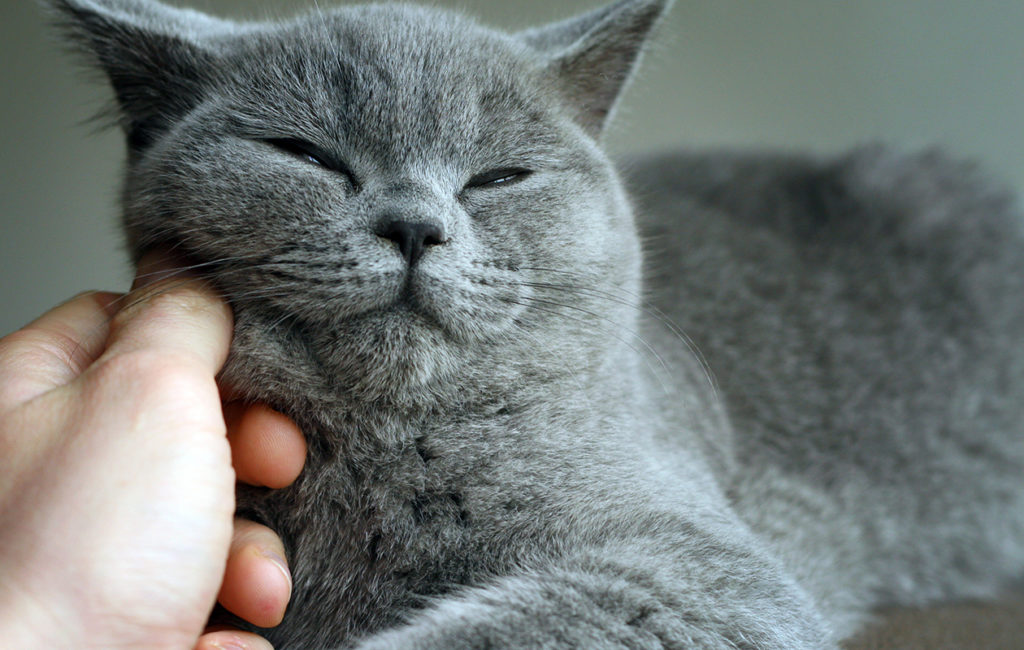
\includegraphics[trim={0cm 0cm 0cm 0cm}, clip, width=\textwidth]{cat}
        \caption{kitty}
        \label{fig:blue}
    \end{subfigure}
    % insert horizontal or vertical spacing here as desired, for example \hspace{-5mm} or \vspace{5mm}
    % easy vertical spacing: \smallskip \medskip
    \hspace{2mm}
    \begin{subfigure}[b]{0.45\textwidth}
        
\includegraphics[trim={0cm 0cm 0cm 0.73cm}, clip, width=\textwidth]{dog}
        \caption{dogo}
        \label{fig:red}
    \end{subfigure}
    \caption[Cat and dog]{Kitty and dogo. Much wow.}
    \label{fig:logos}
\end{figure}

\begin{verbatim}
    You can also use a newline with \\ or \newline to add vertical space.
    Commands are not processed in this verbatim environment.
\end{verbatim}

\subsubsection{Sub-subsection}

This and the following subsections~\ref{subsubsec:another} and~\ref{subsec:third-subsection} demostrate different lists.

Itemize:
\blinditemize

\subsubsection{Another sub-subsection} \label{subsubsec:another}

Enumerate:
\blindenumerate

\subsection{Third subsection} \label{subsec:third-subsection}

Description:
\blinddescription

\clearpage

%%%%%%%%%%%%%%%%%%%%%%%%%%%%%%%%%%%%%%%%%%%%%%%%%%%%%%%%%%%%%%%%%%%%%%%%%%%%%%%%%%%%%%%%%%%%%%%%%%%%%%%%%%%%%%%%%%%%%%%%
%% METHODS

\section{Methods} \label{sec:methods}

Here is some lorem ipsum math stuff.

\blindmathpaper

\clearpage

%%%%%%%%%%%%%%%%%%%%%%%%%%%%%%%%%%%%%%%%%%%%%%%%%%%%%%%%%%%%%%%%%%%%%%%%%%%%%%%%%%%%%%%%%%%%%%%%%%%%%%%%%%%%%%%%%%%%%%%%
%% RESULTS

\section{Results} \label{sec:analysis}

Check appendix~\ref{appendix:extra} for one more figure.

\begin{table}[h]
    \centering
    \renewcommand{\arraystretch}{1.2}
    \setlength{\tabcolsep}{16pt}
    \caption[Example table]{Example table with tabular numbers}
    \begin{tabular}{rrrr}
        \toprule
        \textbf{Col1} & \textbf{Col2} & \textbf{Col2} & \textbf{Col3} \\
        \midrule
        1             & 6             & 87837         & 787           \\
        2             & 005           & 78            & 5415          \\
        3             & 545           & 778           & 7507          \\
        4             & 585           & 18744         & 7560          \\
        5             & 88            & 0788          & 6344          \\
        \bottomrule
    \end{tabular}
    \label{tab:numbers}
\end{table}

\blindtext

Here is an example of \href{https://www.overleaf.com/learn/latex/TikZ_package}{tikz} graphics: \medskip

\begin{figure}[h]
    \centering
    \begin{tikzpicture}[xscale=1.4]
        \draw [very thick] (0,0) -- (10,0);         % horizontal line
        \draw [thick] (0,-.25) -- (0, .25);         % four vertical lines
        \draw [thick] (2.5,-.25) -- (2.5, .25);
        \draw [thick] (7.5,-.25) -- (7.5, .25);
        \draw [thick] (10,-.25) -- (10, .25);
        \node[align=center, below] at (1.25,-.35) {intro part};
        \node[align=center, below] at (5,-.35) {middle part};
        \node[align=center, below] at (8.75,-.35) {outro part};
    \end{tikzpicture}
    \label{fig:tikz}
    \caption[tikz graphics]{Example tikz graphic, which is useful for simple illustrations.}
\end{figure}

\clearpage

%%%%%%%%%%%%%%%%%%%%%%%%%%%%%%%%%%%%%%%%%%%%%%%%%%%%%%%%%%%%%%%%%%%%%%%%%%%%%%%%%%%%%%%%%%%%%%%%%%%%%%%%%%%%%%%%%%%%%%%%
%% DISCUSSION

\section{Discussion} \label{sec:summary}

\blindtext[3]

\clearpage

%%%%%%%%%%%%%%%%%%%%%%%%%%%%%%%%%%%%%%%%%%%%%%%%%%%%%%%%%%%%%%%%%%%%%%%%%%%%%%%%%%%%%%%%%%%%%%%%%%%%%%%%%%%%%%%%%%%%%%%%
%% REFERENCES

% Show all bib entries
% Remove this
\nocite{*}

\addcontentsline{toc}{section}{References}
{
    \interlinepenalty=10000
    \raggedright
    \printbibliography
}

\clearpage

%%%%%%%%%%%%%%%%%%%%%%%%%%%%%%%%%%%%%%%%%%%%%%%%%%%%%%%%%%%%%%%%%%%%%%%%%%%%%%%%%%%%%%%%%%%%%%%%%%%%%%%%%%%%%%%%%%%%%%%%
%% APPENDIX

\appendix
\addcontentsline{toc}{section}{Appendices} \label{sec:appendix}

% Use alphabetic numbering
\renewcommand{\thesubsection}{\Alph{subsection}}

% Reset figure and table counter
\counterwithin{figure}{subsection}
\counterwithin{table}{subsection}

\newgeometry{top=2.5cm, bottom=2cm, left=2.5cm, right=2.5cm}

\subsection{Some extra information} \label{appendix:extra}

Some more dogos in figure~\ref{fig:dogos} in this appendix. \medskip

\begin{figure}[h] % h = here, t = top, b = bottom, H = force here
    \centering
    \begin{subfigure}[b]{0.4\textwidth}
        % crop image -> trim={<left> <lower> <right> <upper>}
        
\includegraphics[trim={0.9cm 0cm 0.9cm 0.73cm}, clip, width=\textwidth]{dog}
        \caption{dogo 1} \vspace{5mm}
    \end{subfigure}
    \hspace{6mm}
    \begin{subfigure}[b]{0.4\textwidth}
        
\includegraphics[trim={0.9cm 0cm 0.9cm 0.73cm}, clip, width=\textwidth]{dog}
        \caption{dogo 2} \vspace{5mm}
    \end{subfigure}
    \begin{subfigure}[b]{0.4\textwidth}
        \scalebox{1}[-1]{
\includegraphics[trim={0.9cm 0cm 0.9cm 0.73cm}, clip, width=\textwidth]{dog}}
        \caption{dogo 3: vertical flip}
    \end{subfigure}
    \hspace{6mm}
    \begin{subfigure}[b]{0.4\textwidth}
        \scalebox{-1}[1]{
\includegraphics[trim={0.9cm 0cm 0.9cm 0.73cm}, clip, width=\textwidth]{dog}}
        \caption{dogo 4: horizontal flip}
    \end{subfigure}
    \caption[More dogs]{Wow, more dogos.}
    \label{fig:dogos}
\end{figure}

\end{document}
